% -*- TeX:de -*-
\NeedsTeXFormat{LaTeX2e}
\documentclass[12pt,a4paper,titlepage]{article}

%\usepackage[german]{babel} % german text
\usepackage[DIV12]{typearea} % size of printable area
\usepackage[T1]{fontenc} % font encoding
\usepackage[utf8]{inputenc} % probably on Linux

\usepackage{graphicx} % to include images
\graphicspath{ {img/} } % set default image directory
\usepackage{subfigure} % for creating subfigures
\usepackage{amsmath} % a bunch of symbols
\usepackage{amssymb} % even more symbols
\usepackage{booktabs} % pretty tables
\usepackage{csquotes}

% a floating environment for circuits
\usepackage{float}
\usepackage{caption}

\newfloat{circuit}{tbph}{circuits}
\floatname{circuit}{Schaltplan}

% a floating environment for diagrams
\newfloat{diagram}{tbph}{diagrams}
\floatname{diagram}{Diagramm}

\renewcommand{\familydefault}{\sfdefault} % activate to use sans-serif font as default

\sloppy % friendly typesetting

\usepackage{eurosym}
\usepackage{makeidx}
\usepackage{amsfonts}
\usepackage{mparhack}
\usepackage{array}
\usepackage{tabularx}
\usepackage{minitoc}
\usepackage[colorlinks=true]{hyperref}
\usepackage{epstopdf}
\usepackage{setspace}
\usepackage{csquotes}

% hyperref settings
\hypersetup{
    colorlinks=false,       % false: boxed links; true: colored links
    linkcolor=black,          % color of internal links (change box color with linkbordercolor)
    citecolor=black,        % color of links to bibliography
    filecolor=black,      % color of file links
    urlcolor=black           % color of external links
}

\begin{document}

\begin{titlepage}

\begin{figure*}[h!]
  
\includegraphics[width=8cm]{TULogo_CMYK}
\end{figure*}

\begin{center}
\vspace*{1.3cm}
{\Huge Elektrotechnische Grundlagen der Informatik\\(LU 182.692)\\}
\vspace{1.7cm}
{\LARGE Protokoll der 3. Laborübung: \enquote{Operationsverstärker}\\}
{\LARGE  a) LTSPICE-Simulationen\\}
\vspace{1.7cm}

% fill in group number and date of lab here
% CHANGE ME!
{\Large Gruppennr.: 22 \hspace{1cm} Datum der Labor\"ubung: 01.06.2017}

% fill in IDs and names here
% CHANGE ME!
\begin{table}[h!]
\centering
\begin{tabular}{|p{3.5cm}|p{3.5cm}|p{6.5cm}|}
\hline \textbf{Matr. Nr.} & \textbf{Kennzahl} & \textbf{Name} \\
\hline
1614835 & 033 535 & Jan Nausner \\
\hline
1633068 & 033 535 & David Pernerstorfer \\
\hline
\end{tabular}
\end{table}

\end{center}
\vspace{1.0cm}

\begin{table}[h!]
\begin{tabular}{|l|l|}
\hline \textbf{Kontrolle} & \checkmark \\
\hline Nichtinvertierender OPV & \\
\hline OPV und Grenzfrequenz & \\
\hline Invertierender OPV & \\
\hline Integrierer & \\
\hline Schmitt-Trigger & \\
\hline
\end{tabular}
\end{table}

\end{titlepage}
% start of actual lab protocol
% CHANGE ME!

\setcounter{page}{2}

\newpage
\setcounter{tocdepth}{1}
\tableofcontents

\newpage



\section{Nichtinvertierender Verst\"arker}

\subsection{Aufgabenstellung}
Das Verhalten eines OPV als nichtinvertierender Verst\"arker soll mittels LTSpice simuliert werden.

\subsection{Schaltplan}
\begin{figure}[H]
  \centering
  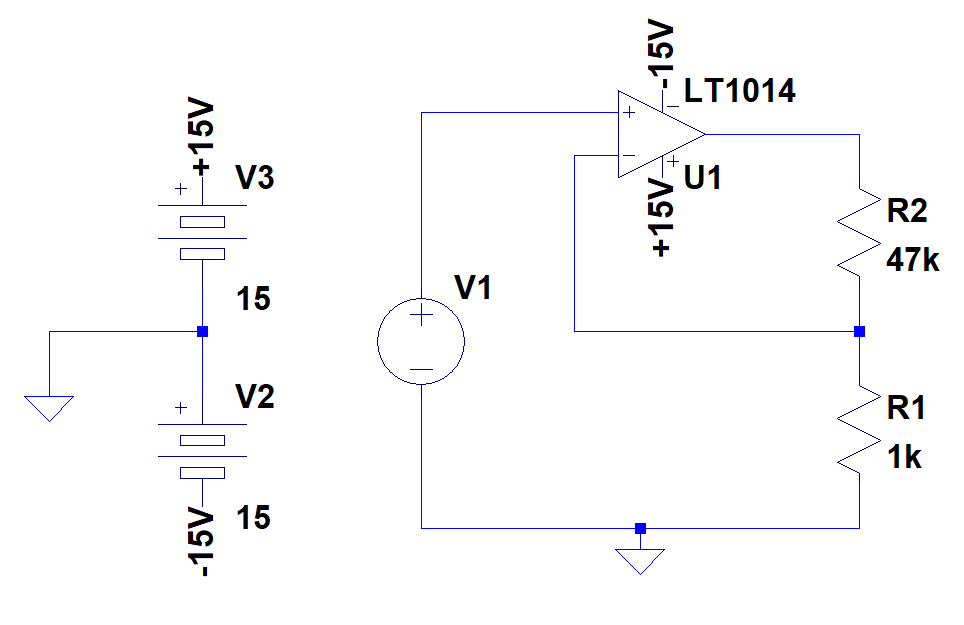
\includegraphics{nichtinvertierend_schaltung}
  \caption{Nichtinvertierender Verst\"arker}
  \label{figure01}
\end{figure}

\subsection{Durchf\"uhrung}
Die Schaltung eines OPV als nichtinvertierender Verst\"arker wurde mit LTSpice aufgebaut (Abbildung~\ref{figure01}). Die Spannungsverst\"arkung wird mit $V_u = 1 + \frac{R_2}{R_1}$ berechnet und soll zwischen $40$ und $60$ liegen. Das bedeutet $R_2$ muss etwa $40$ bis $60$ mal gr\"o\ss er dimensioniert werden als $R_1$. Gew\"ahlt wurden die Widerst\"ande $R_1 = 1k\Omega$ und $R_2 = 47k\Omega$. Nun wurde das Verhalten des Systems mit einer DC Eingangsspannung bzw. mit 2 verschieden Rechteckspannungen (siehe Angabe) simuliert und diverse Messungen durchgef\"uhrt (siehe Ergebnis \& Diskussion).


\subsection{Ergebnis \& Diskussion}
\begin{table}[H]
\centering
\begin{tabular}{|l|l|l|}
\hline
Strom Widerstand $R_1$ & $I_{R1}$ & $100,00\mu A$  \\ \hline
Strom Widerstand $R_2$ & $I_{R2}$ & $99,99\mu A$  \\ \hline
Spannung Widerstand $R_1$ & $U_{R1}$ & $100,00mV$  \\ \hline
Spannung Widerstand $R_2$ & $U_{R2}$ & $4,70V$ \\ \hline
% positive Eingansspannung OPV & $U_p$  & $100mV$        \\ \hline
% negative Eingangsspannung OPV & $U_n$  & $99,999309mV$  \\ \hline
Spannungsdifferenz Eingang OPV & $U_d$  & $0,69\mu V$      \\ \hline
Strom Eingang OPV & $I_d$  & $12,01nA$ \\ \hline
Eingangsspannung & $U_e$  & $100mV$        \\ \hline
Ausgangsspannung & $U_a$  & $4,80V$   \\ \hline
\end{tabular}
\caption{Messwerte Nichtinvertierender Verst\"arker bei DC 0,1V}
\label{figure02}
\end{table}
In Abbildung~\ref{figure02} sind die Messwerte des OPVs als nichtinvertierender Verst\"arker mit einer Gleichspannung von $100mV$ zu sehen. Grunds\"atzlich w\"are die Verst\"arkung eines OPVs unendlich gro\ss \, und die Verst\"arkung w\"urde bei wenigen $\mu V$ die positive bzw. negative Versorungsspannung annehmen. Jedoch wird ein Teil der Ausgangsspannung an den invertierenden Eingang des OPVs zur\"uckgef\"uhrt (Gegenkopplung), dadurch kann die Verst\"arkung geregelt werden. Aufgrund des im Idealfall unendlich gro\ss en Eingangswiderstands am OPV flie\ss t zwischen den Eing\"angen verschwindend geringer Strom ($12,01nA$). Aufgrund der Knotenregel flie\ss t daher an $R_1$ und $R_2$ praktisch der gleiche Strom. Weiters ist aufgrund der Maschenregel $U_{R1} = U_e$ und $U_a = U_{R2} + U_{R1}$. Aus diesen Aussagen kann nun die Verst\"arkung des Systems hergeleitet und berechnet werden.\\
\begin{equation*}
  V = \frac{U_a}{U_e} = \frac{U_{R1} + U_{R2}}{U_{R1}} = \frac{R_1 + R_2}{R_1} = 1+ \frac{R_2}{R_1} \\
\end{equation*}
\begin{equation*}
  V = 1 + \frac{47 k\Omega}{1 k\Omega} = 48
\end{equation*}
\noindent Die berechnete Verst\"arkung passt mit den gemessen Werten \"uberein ($U_e = 100mV$, $U_a = 4,80V$).

\begin{figure}[H]
  \centering
  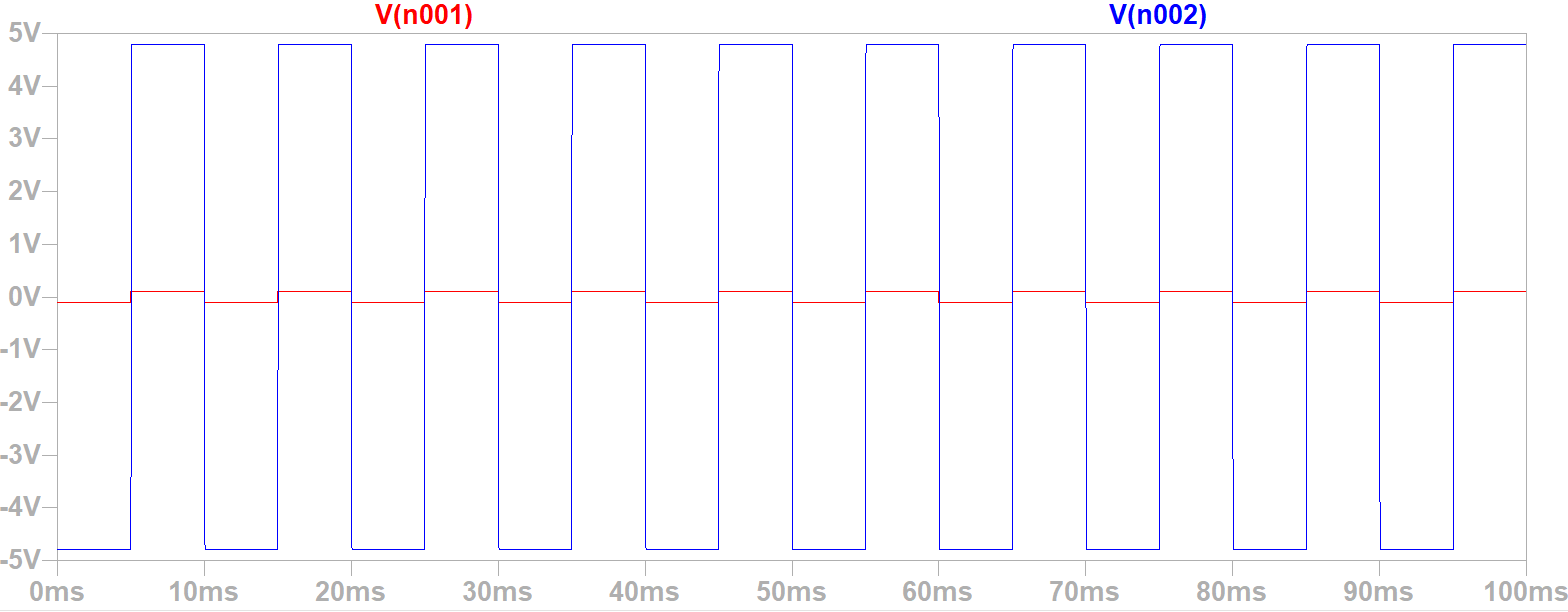
\includegraphics[width=150mm]{nichtinvertierend_pulse_eingangs_ausgangsspannung}
  \caption{Nichtinvertierender Verst\"arker mit Rechtecksignal $100Hz$; Blau: Ausgangsspannung $U_a$; Rot: Eingangsspannung $U_e$}
  \label{figure03}
\end{figure}
<<<<<<< HEAD
Die Abbildung~\ref{figure03} zeigt Eingangs- und Ausgangsspannung ($U_e$ und $U_a$) des Nichtinvertierendne Verst\"arkers mit einem Recktecksignal von $100Hz$ und $100mV$ Spannungsamplitude am Eingang. Die gemessene Amplitude der Ausgangsspannug von $4,80V$ entspricht wieder der erwarteten Verst\"arkung von $V = 48$. Wie zu erkennen ist, sind Eingangs- und Ausgangsspannung phasengleich.
=======
In Abbildung~\ref{figure01} sind die Spannungen des positiven ($U_p$) und negativen ($U_n$) Einganges des OPV zu sehen. $U_p$ entspricht klarerweise der Eingangsspannung $U_e$. Da zwischen den beiden Eing\"angen
>>>>>>> d7ec21a920cc48ffb4915775081ee2cd6bdc861f

\begin{figure}[H]
  \centering
  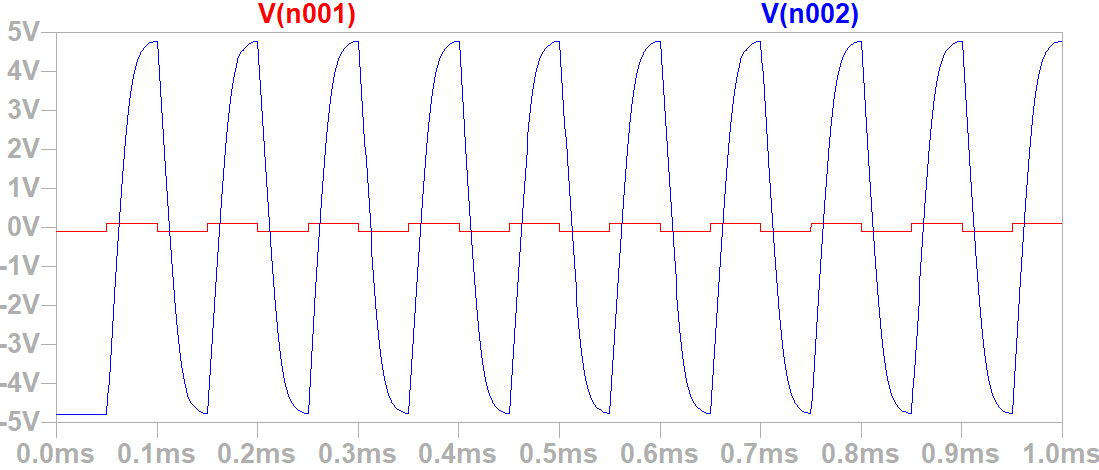
\includegraphics[width=150mm]{nichtinvertierend_pulse2_eingangs_ausgangsspannung}
  \caption{Nichtinvertierender Verst\"arker mit Rechtecksignal $10kHz$; Blau: Ausgangsspannung $U_a$; Rot: Eingangsspannung $U_e$}
  \label{figure04}
\end{figure}
Die Abbildung~\ref{figure03} zeigt Eingangs- und Ausgangsspannung ($U_e$ und $U_a$) des Nichtinvertierendne Verst\"arkers mit einem Recktecksignal von $10kHz$ und $100mV$ Spannungsamplitude am Eingang. Die gemessene Amplitude der Ausgangsspannung von $4,80V$ entspricht wieder erwarteten Verst\"arkung von $V = 48$. Aufgrund der inneren Kapazit\"at des OPVs verh\"ahlt sich das Ausgangssignal \"ahnlich wie ein Tiefpass 1.Ordnung (RC-Glied). Diese Kurvenform wird nur bei h\"oherer Frequenz sichtbar.

\section{Invertierender Verst\"arker}

\subsection{Aufgabenstellung}
Das Verhalten eines OPV als invertierender Verst\"arker soll mittels LTSpice simuliert werden.

\subsection{Schaltplan}
\begin{figure}[H]
  \centering
  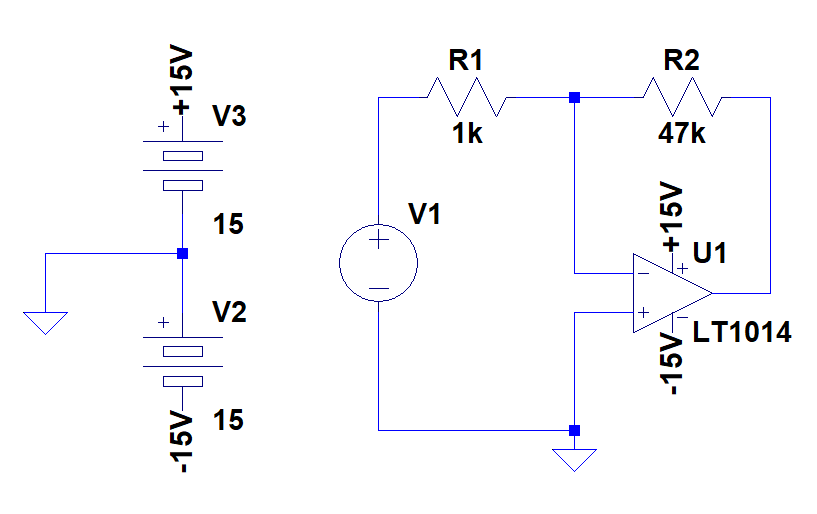
\includegraphics{invertierend_schaltung}
  \caption{Invertierender Verst\"arker}
  \label{figure11}
\end{figure}

\subsection{Durchf\"uhrung}
Die Schaltung eines OPV als invertierender Verst\"arker wurde mit LTSpice aufgebaut (Abbildung~\ref{figure11}). Die Spannungsverst\"arkung wird mit $V_u = -\frac{R_2}{R_1}$ berechnet und soll zwischen $-40$ und $-60$ liegen. Das bedeutet $R_2$ muss $40$ bis $60$ mal gr\"o\ss er dimensioniert werden als $R_1$. Gew\"ahlt wurden die Widerst\"ande $R_1 = 1k\Omega$ und $R_2 = 47k\Omega$. Nun wurde das Verhalten des Systems mit einer DC Eingangsspannung bzw. mit Dreiecksignal mit Frequenz $100Hz$ und $10kHz$ simuliert. Weiters wurde der Frequenzbereich $1Hz$ bis $10MHz$ mit Sinussignal und $V_{PP} = 0.1V$ simuliert und ein Bodediagramm geplottet. Die selbe Simulation sollte f\"ur die gleiche Schaltung mit einer Verst\"arkung von $-4$ bis $-6$ durgef\"uhrt werden. Dazu wurden die Widerst\"ande $R_1 = 1k\Omega$ und $R_2 = 4,7k\Omega$ gew\"ahlt, was eine Verst\"arkung von $V_u = -\frac{4,7k\Omega}{1k\Omega} = -4,7$ ergibt. Die Digramme und Eregebnisse sind im Abschnitt \textit{Ergebnis \& Diskussion} zu finden. \\

\subsection{Ergebnis \& Diskussion}
\begin{table}[H]
\centering
\begin{tabular}{|l|l|l|}
\hline
Strom Widerstand $R_1$ & $I_{R1}$ & $100,00\mu A$  \\ \hline
Strom Widerstand $R_2$ & $I_{R2}$ & $100,01\mu A$  \\ \hline
Spannung Widerstand $R_1$ & $U_{R1}$ & $100,00mV$  \\ \hline
Spannung Widerstand $R_2$ & $U_{R2}$ & $-4,70V$ \\ \hline
% positive Eingansspannung OPV & $U_p$  & $100mV$        \\ \hline
% negative Eingangsspannung OPV & $U_n$  & $99,999309mV$  \\ \hline
Spannungsdifferenz Eingang OPV & $U_d$  & $0,68\mu V$      \\ \hline
Strom Eingang OPV & $I_d$  & $12,02nA$ \\ \hline
Eingangsspannung & $U_e$  & $100mV$        \\ \hline
Ausgangsspannung & $U_a$  & $-4,70V$   \\ \hline
\end{tabular}
\caption{Messwerte Invertierender Verst\"arker bei DC 0,1V}
\label{figure12}
\end{table}
In Abbildung~\ref{figure12} sind die Messwerte des OPVs als invertierender Verst\"arker mit einer Gleichspannung von $100mV$ zu sehen. Grunds\"atzlich w\"are die Verst\"arkung eines OPVs $-\infty$ und die Verst\"arkung w\"urde bei wenigen $\mu V$ die positive bzw. negative Versorungsspannung annehmen, und zwar jeweils negiert zur Spannung am invertierenden Eingang. Jedoch wird durch die Gegenkopplung (OPV Ausgang ist verbunden mit invertierenden Eingang) die Verst\"arkung durch die beiden Widerst\"ande geregelt. Da ein OPV versucht die Spannungen an den Eing\"angen gleich zu halten und der nichtinvertierende Eingang mit Masse verbunden ist, hat man am invertierenden Eingang einen sog. \"virtuellen Nullpunkt\". Da der Eingangswiderstand am OPV sehr gro\ss \, (im Idealfall unendlich) ist, flie\ss t kaum Strom zwischen den beiden Eing\"angen ($12,02nA$). Da $R_1$ einerseits mit der Spannungsquelle und andererseits mit dem virtuellen Nullpunkt (Masse) verbunden ist, kann man $U_{R1}$ gleich $U_e$ setzen. Aus dem gleichen Grund kann man $U_{R1}$ gleich $U_a$ setzen. Weiters kann man aufgrund der Knotenregel den Strom am $R_1$ und $R_2$ gleich setzen. Aus diesen Aussagen kann nun die Verst\"arkung des Systems hergeleitet werden.
\begin{equation*}
  V = -\frac{U_a}{U_e} = -\frac{U_{R2}}{U_{R1}} = -\frac{R_2}{R_1} \\
\end{equation*}
\begin{equation*}
  V = -\frac{47 k\Omega}{1 k\Omega} = 47
\end{equation*}
\noindent Die berechnete Verst\"arkung passt mit den gemessen Werten \"uberein ($U_e = 100mV$, $U_a = -4,70V$).

\begin{figure}[H]
  \centering
  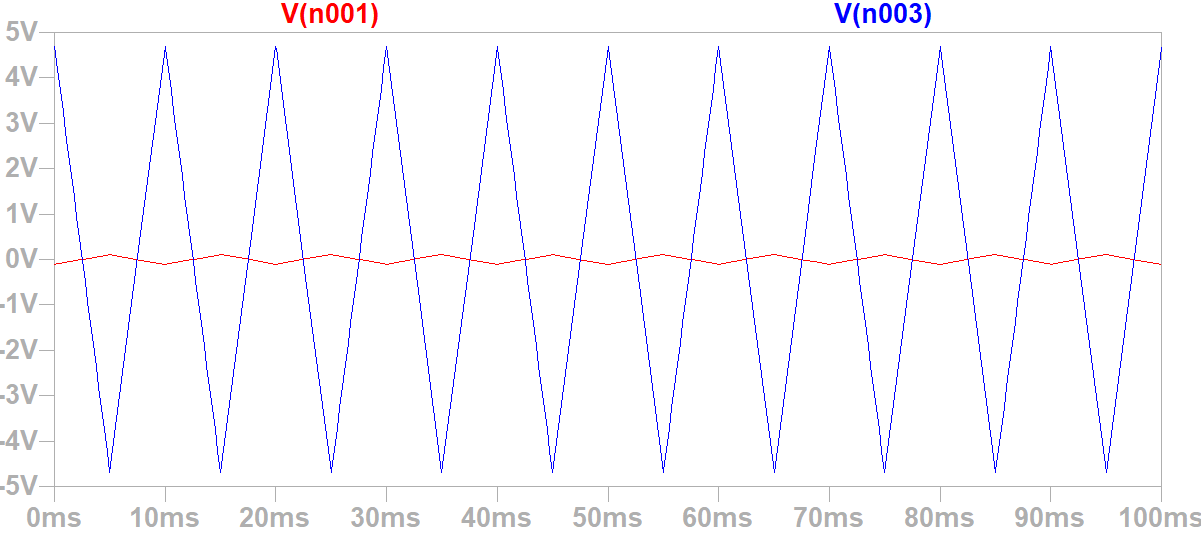
\includegraphics[width=150mm]{invertierend_dreieck_eingangs_ausgangsspannung}
  \caption{Invertierender Verst\"arker mit Dreiecksignal $100Hz$; Blau: Ausgangsspannung $U_a$; Rot: Eingangsspannung $U_e$}
  \label{figure13}
\end{figure}

\begin{figure}[H]
  \centering
  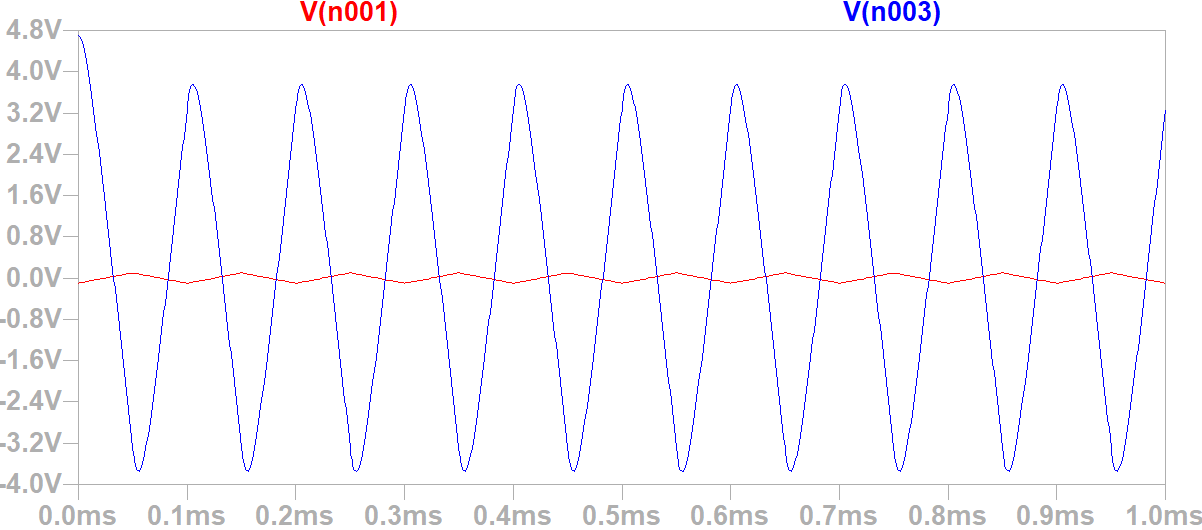
\includegraphics[width=150mm]{invertierend_dreieck2_eingangs_ausgangsspannung}
  \caption{Invertierender Verst\"arker mit Dreiecksignal $10kHz$; Blau: Ausgangsspannung $U_a$; Rot: Eingangsspannung $U_e$}
  \label{figure14}
\end{figure}

\begin{figure}[H]
  \centering
  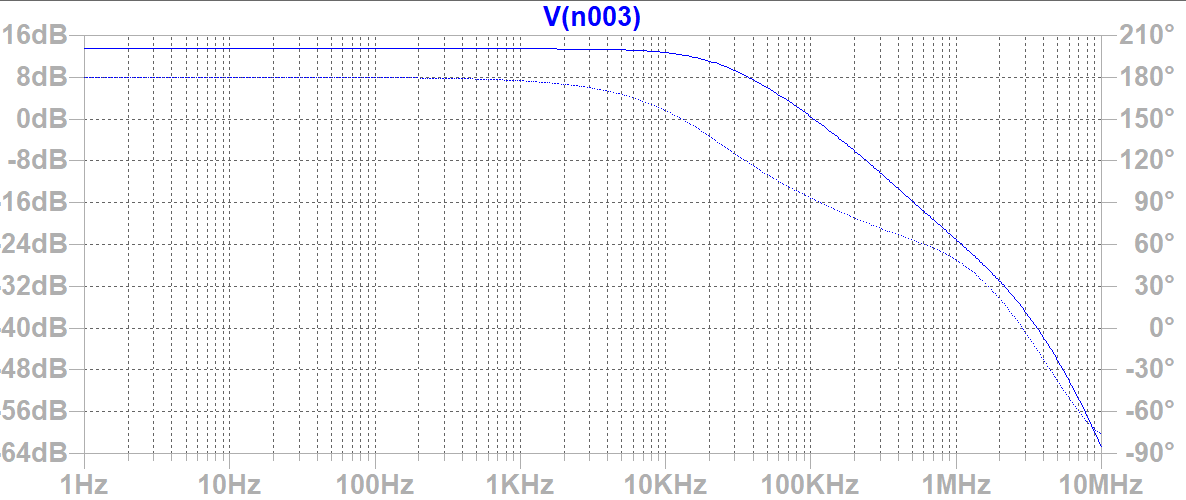
\includegraphics[width=150mm]{invertierend_bode1}
  \caption{Invertierender Verst\"arker Bodediagramm}
  \label{figure15}
\end{figure}

\begin{figure}[H]
  \centering
  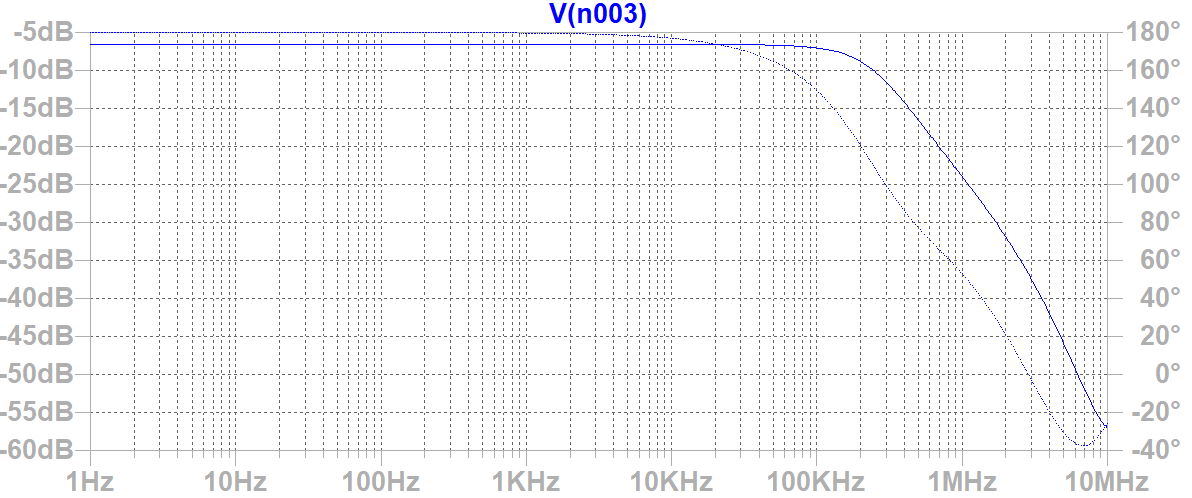
\includegraphics[width=150mm]{invertierend_bode2}
  \caption{Invertierender Verst\"arker Bodediagramm}
  \label{figure16}
\end{figure}





\section{Integrierer}

\subsection{Aufgabenstellung}
Das Verhalten eines Integrierers soll im Zeit- und Frequenzbereich simuliert werden.

\subsection{Schaltplan}
\begin{figure}[H]
  \centering
  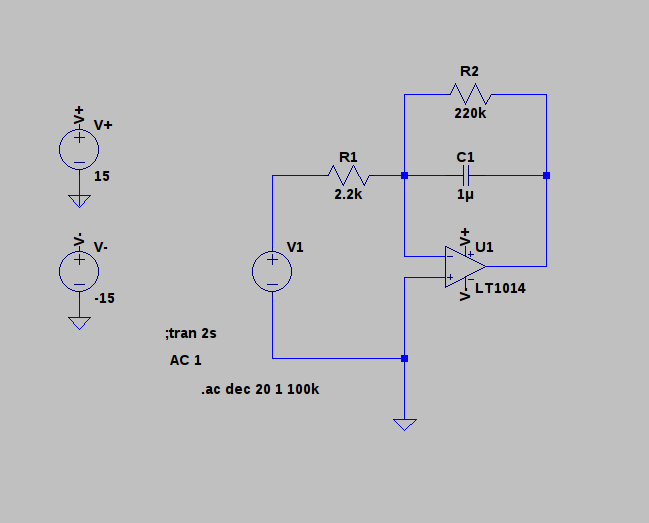
\includegraphics[width=100mm]{integrierer_schaltung.png}
  \caption{Integrierer}
\end{figure}

\subsection{Durchf\"uhrung}
Die Schaltung wurde gem\"aß Angabe zusammengef\"ugt. Die Versorgungsspannung des OPV (LT1014) betr\"agt $\pm 15V$. Um das Verhalten im Zeitbereich zu simulieren, wurde eine Rechteckspannung mit $f=5Hz, A=\pm 0,1V, V_{initial}=-0,1V$ angelegt. Das Zeitverhalten wurde im Bereich von $0$ bis $2s$ aufgezeichnet. Zur Simulation des Frequenzverhaltens wurde eine Sinusspannung mit $1V_{pp}$ angelegt und das Bode-Diagramm von $1Hz-100kHz$ aufgezeichnet.

\subsection{Ergebnis \& Diskussion}

\begin{figure}[H]
  \centering
  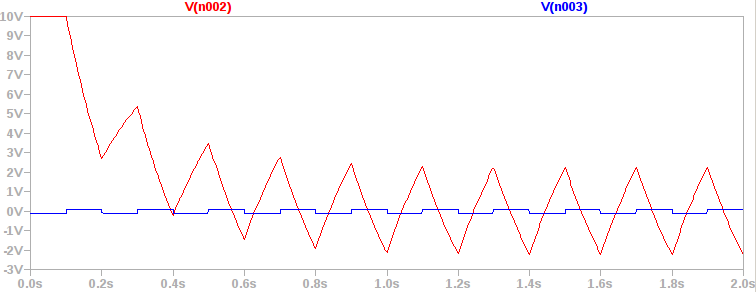
\includegraphics[width=150mm]{integrierer_transient.png}
  \caption{Zeitverhalten (rot $\hdots$ Ausgangsspannung, blau $\hdots$ Eingangsspannung)}
\end{figure}
Im Bereich von $0$ bis $1s$ ist ein Einschwingvorgang zu erkennen, welcher auf das $RC$-Glied zur\"uckzuf\"uhren ist. Da die Differenz der beiden OPV-Eing\"ange zu Beginn $-0,1V$ Betr\"agt, \"ubersteuert der OPV, die Differenz schl\"agt auf $0,1V$ um und der OPV versucht zu untersteuern, dann pendelt sich das Signal ein. Im eingeschwungenenen Zustand wird das anliegende Rechtecksignal gem\"aß der \"Ubertragungsfunktion

\begin{figure}[H]
  \centering
  $U_a = -\frac{1}{RC}\int U_e dt$
\end{figure}

\noindent zu einem Dreieckssignal mit

\begin{figure}[H]
  \centering
  $U_e<0: U_a = \frac{t}{10*RC} \approx 45,5*t, U_e>0: U_a = -\frac{t}{10*RC} \approx -45,5*t$
\end{figure}

\noindent integriert. TODO: Anfangsbedingung, Vpp!!!


\begin{figure}[H]
  \centering
  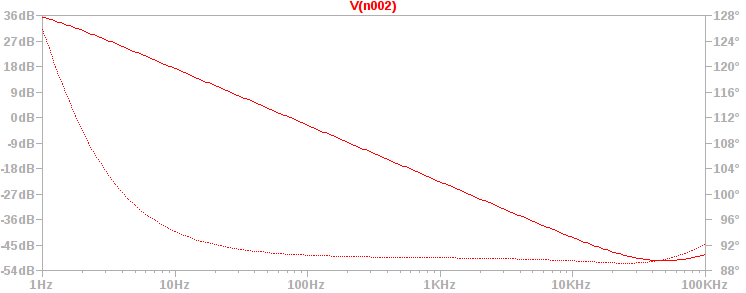
\includegraphics[width=150mm]{integrierer_bode.png}
  \caption{Bode-Diagramm}
\end{figure}

\noindent Am Frequenzverhalten kann man erkennen, dass das System bis zur Grenzfrequenz des $RC$-Glieds ($f_g = \frac{1}{2\pi RC} \approx 72Hz$) verst\"arkend wirkt und danach zu D\"ampfen beginnt. Die Filtersteilheit betr\"agt $-20dB/Dekade$. Die Phase dreht zuerst sehr stark, dann immer schw\"acher von $126^{\circ}$ auf $90^{\circ}$. Im Bereich \"uber $40kHz$ beginnt die Phasenverschiebung wieder zu steigen und die D\"ampfung wird schw\"acher.\\

\noindent TODO: grober Unfug?

\section{Invertierender Schmitt-Trigger}

\subsection{Aufgabenstellung}
Das Verhalten eines invertierenden Schmitt-Triggers soll im Zeitbereich simuliert werden.

\subsection{Schaltplan}
\begin{figure}[H]
  \centering
  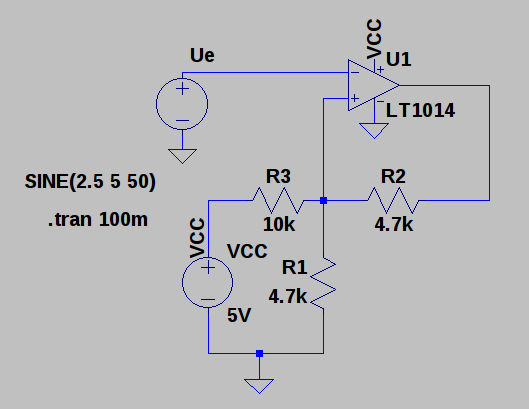
\includegraphics[width=100mm]{schmitt_schaltung.png}
  \caption{Invertierender Schmitt-Trigger}
\end{figure}

\subsection{Durchf\"uhrung}
Die Schaltung wurde gem\"aß Angabe zusammengef\"ugt. Die Versorgungsspannung des OPV (LT1014) betr\"agt $V+=5V,V-=0V$. Zuerst wurde die Aus- und Eingangsspannung, sowie die Spannung am positiven Eingang des OPV im Bereich von $0$ bis $100ms$ mit einem Sinus-Eingangssignal ($DC_{offset} = 2,5V, V_{pp} = 5V, f = 50Hz$) simuliert. Dann wurde das Zeitverhalten mit einem Dreieckssignal ($V_{on} = 5V, V_{off} = 0V, f = 5MHz$) von $0$ bis $1\mu s$ simuliert.

\subsection{Ergebnis \& Diskussion}

\begin{figure}[H]
  \centering
  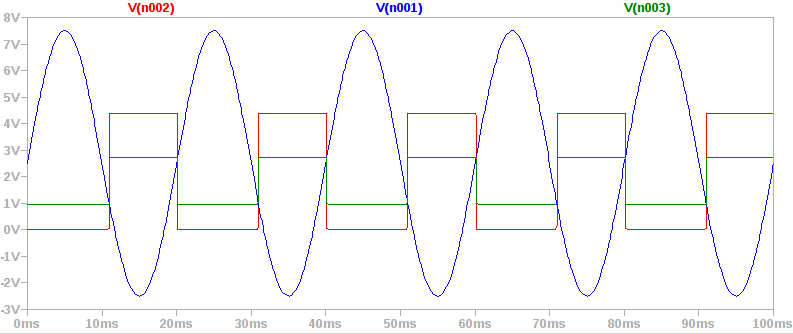
\includegraphics[width=150mm]{schmitt_transient.png}
  \caption{Zeitverhalten bei Sinussignal (rot $\hdots$ Ausgangsspannung, blau $\hdots$ Eingangsspannung, gr\"un $\hdots$ Spannung am positiven OPV Eingang)}
\end{figure}

\noindent Berechnung der Spannung am positiven OPV Eingang mittels Superpositionsprinzip:

\begin{itemize}
  \item $U_{low} = 0,029V$ (abgelesen):\\
  $U_a$ kurzgeschlossen:\\
  $U_{p1} = U_{VCC}\frac{R_{12}}{R_{12}+r_3} = U_{VCC}\frac{\frac{R_1R_2}{R_1+R_2}}{\frac{R_1R_2}{R_1+R_2}+R_3} = 5V\frac{2,35k\Omega}{2,35k\Omega + 10k\Omega} \approx 0,95V$\\
  $U_{VCC}$ kurzgeschlossen:\\
  $U_{p2} = U_{low}\frac{R_{13}}{R_{13}+R_2} = U_{low}\frac{\frac{R_1R_3}{R_1+R_3}}{\frac{R_1R_3}{R_1+R_3}+R_2} = 0,029V\frac{3,19k\Omega}{3,19k\Omega + 4,7k\Omega} \approx 0,01V$\\
  $U_p = U_{p1} + U_{p2} \approx 0,96V$

  \item $U_{high} = 4,39V$ (abgelesen):\\
  $U_a$ kurzgeschlossen:\\
  $U_{p1} = U_{VCC}\frac{R_{12}}{R_{12}+R_3} = U_{VCC}\frac{\frac{R_1R_2}{R_1+R_2}}{\frac{R_1R_2}{R_1+R_2}+R_3} = 5V\frac{2,35k\Omega}{2,35k\Omega + 10k\Omega} \approx 0,95V$\\
  $U_{VCC}$ kurzgeschlossen:\\
  $U_{p2} = U_{high}\frac{R_{13}}{R_{13}+R_2} = U_{high}\frac{\frac{R_1R_3}{R_1+R_3}}{\frac{R_1R_3}{R_1+R_3}+R_2} = 4,39V\frac{3,19k\Omega}{3,19k\Omega + 4,7k\Omega} \approx 1,78V$\\
  $U_p = U_{p1} + U_{p2} \approx 2,73V$
\end{itemize}

\noindent Die Spannung am positiven Eingang des OPV bestimmt (wie auch im Diagramm ersichtlich), wann getriggert wird. Das heißt, wenn das Sinussignal am Eingang unter $0,95V$ f\"allt, liefert der OPV am Ausgang $U_{high}$, wenn das Eingangssignal $2,73V$ \"ubersteigt, liegt am Ausgang $U_{low}$ an. Somit wandelt der Schmitt-Trigger das Sinussignal in ein invertiertes Rechtecksignal um.

\begin{figure}[H]
  \centering
  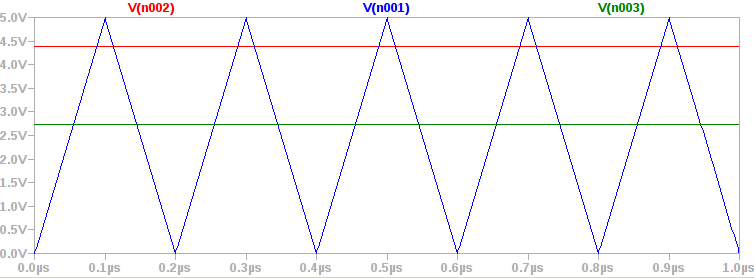
\includegraphics[width=150mm]{schmitt_transient2.png}
  \caption{Zeitverhalten bei $5MHz$ Dreieckssignal (rot $\hdots$ Ausgangsspannung, blau $\hdots$ Eingangsspannung, gr\"un $\hdots$ Spannung am positiven OPV Eingang)}
\end{figure}

\noindent Durch die hohe Frequenz des Eingangssignals wird der verwendete OPV an seine Grenzen getrieben und kann nicht mehr schnell genug schalten. Das gew\"unschte Schmitt-Trigger-Verhalten ist nicht mehr zu erkennen.

\end{document}
